\section{Preventivo}
Per descrivere come il gruppo \emph{TechSWEave} utilizzerà le risorse a sua disposizione, abbiamo stilato delle tabelle orarie con la suddivisione dei ruoli, utilizzando le seguenti sigle:
\begin{itemize}
    \item \textbf{Re: }\emph{Responsabile};
    \item \textbf{Am: }\emph{Amministratore}
    \item \textbf{An: }\emph{Analista};
    \item \textbf{Pt: }\emph{Progettista};
    \item \textbf{Pr: }\emph{Programmatore};
    \item \textbf{Ve: }\emph{Verificatore};
\end{itemize}

\subsection{Fase di Analisi}
\subsubsection{Prospetto orario}
In questa periodo la distribuzione oraria dei ruoli sarà la seguente:
\begin{center}
    \begin{table}[ht!]
        \centering
        \caption{Distribuzione delle ore della fase di Analisi}
        \vspace{5px}
        \rowcolors{2}{logo!10}{logo!40}
        \renewcommand{\arraystretch}{1.8}
        \begin{tabular}{p{100px} p{20px} p{20px} p{20px} p{20px} p{20px} p{20px} p{50px} }
            \rowcolor{logo!70} \textbf{Nominativo} & \textbf{Re} & \textbf{Am} & \textbf{An} & \textbf{Pt} & \textbf{Pr} & \textbf{Ve} & \textbf{Ore totali} \\
            Marco Barbaresco                       & -           & 10          & 10          & -           & -           & 15          & 35                  \\
            Samuele De Simone                      & 8           & -           & 17          & -           & -           & 10          & 35                  \\
            Nicolò Giaccone                        & -           & 7           & 21          & -           & -           & 7           & 35                  \\
            Amedeo Meggiolaro                      & -           & -           & 18          & -           & -           & 17          & 35                  \\
            Tito Scutari                           & -           & 8           & 12          & -           & -           & 15          & 35                  \\
            Simone Urbani                          & 6           & 10          & 8           & -           & -           & 11          & 35                  \\
            Manuel Varo                            & 7           & -           & 12          & -           & -           & 16          & 35                  \\
            Ore totali di ruolo                    & 21          & 35          & 98          & -           & -           & 91          & 245                 \\
        \end{tabular}
    \end{table}
\end{center}

\pagebreak
I dati appena descritti si possono riassumere nel seguente istogramma:
\begin{figure}[!h]
    \vspace{5px}
    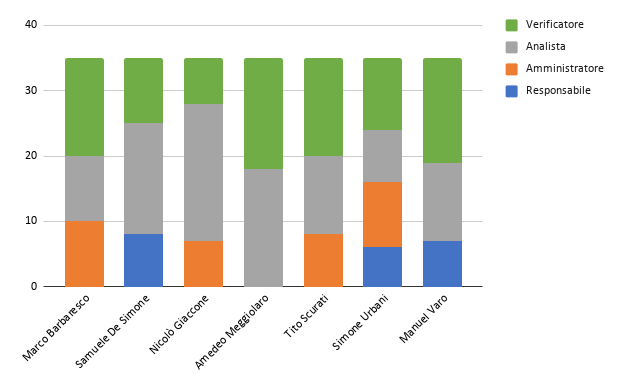
\includegraphics[scale=0.6]{../../../Images/Diagrammi/Istogrammi/ore analisi.png}
    \centering
    \caption{Istogramma della suddivisione delle ore per ruolo nell' Analisi}
\end{figure}
\subsubsection{Prospetto economico}
In questa fase i costi da affrontare per ogni ruolo sono i seguenti:
\begin{center}
    \begin{table}[ht!]
        \centering
        \caption{Prospetto dei costi per ruolo nel periodo di Analisi}
        \vspace{5px}
        \rowcolors{2}{logo!10}{logo!40}
        \renewcommand{\arraystretch}{1.8}
        \begin{tabular}{p{75px} p{20px} p{50px} }
            \rowcolor{logo!70} \textbf{Ruolo} & \textbf{Ore} & \textbf{Costo}  \\
            Responsabile                      & 21           & 630,00\EURdig   \\
            Amministratore                    & 35           & 700,00\EURdig   \\
            Analista                          & 98           & 2.450,00\EURdig \\
            Progettista                       & -            & -               \\
            Programmatore                     & -            & -               \\
            Verificatore                      & 91           & 1.365,00\EURdig \\
            Totale                            & 245          & 5.145,00\EURdig \\
        \end{tabular}
    \end{table}
\end{center}
\pagebreak
I dati appena descritti si possono riassumere nel seguente areogramma:
\begin{figure}[!h]
    \vspace{5px}
    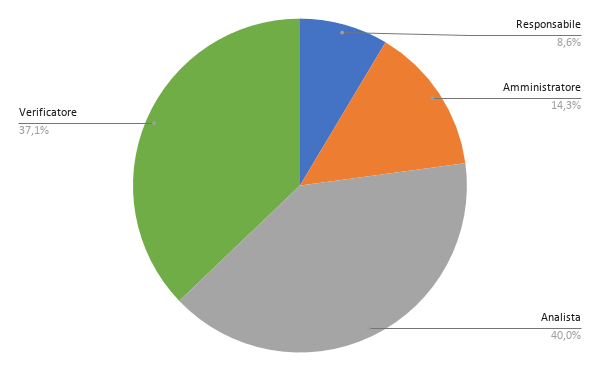
\includegraphics[scale=0.5]{../../../Images/Diagrammi/Diagramma a torta/ore analisi.png}
    \centering
    \caption{Areogramma della suddivisione di ore per ruolo in Analisi}
\end{figure}


\subsection{Fase di Consolidamento dei requisiti}
\subsubsection{Prospetto orario}
Per il periodo di Consolidamento dei requisiti la suddivisione oraria dei ruoli sarà la seguente:

\begin{center}
    \begin{table}[ht!]
        \centering
        \caption{Distribuzione delle ore della fase di Consolidamento dei requisiti}
        \vspace{5px}
        \rowcolors{2}{logo!10}{logo!40}
        \renewcommand{\arraystretch}{1.8}
        \begin{tabular}{p{100px} p{20px} p{20px} p{20px} p{20px} p{20px} p{20px} p{50px} }
            \rowcolor{logo!70} \textbf{Nominativo} & \textbf{Re} & \textbf{Am} & \textbf{An} & \textbf{Pt} & \textbf{Pr} & \textbf{Ve} & \textbf{Ore totali} \\
            Marco Barbaresco                       & -           & -           & 2           & -           & -           & 4           & 6                   \\
            Samuele De Simone                      & 4           & -           & -           & -           & -           & 2           & 6                   \\
            Nicolò Giaccone                        & -           & -           & 6           & -           & -           & -           & 6                   \\
            Amedeo Meggiolaro                      & -           & -           & -           & -           & -           & 6           & 6                   \\
            Tito Scutari                           & -           & -           & 6           & -           & -           & -           & 6                   \\
            Simone Urbani                          & -           & 6           & -           & -           & -           & -           & 6                   \\
            Manuel Varo                            & -           & -           & 2           & -           & -           & 4           & 6                   \\
            Ore totali di ruolo                    & 4           & 6           & 16          & -           & -           & 16          & 42                  \\
        \end{tabular}
    \end{table}
\end{center}
\pagebreak

I dati appena descritti si possono riassumere nel seguente istogramma:
\begin{figure}[!h]
    \vspace{5px}
    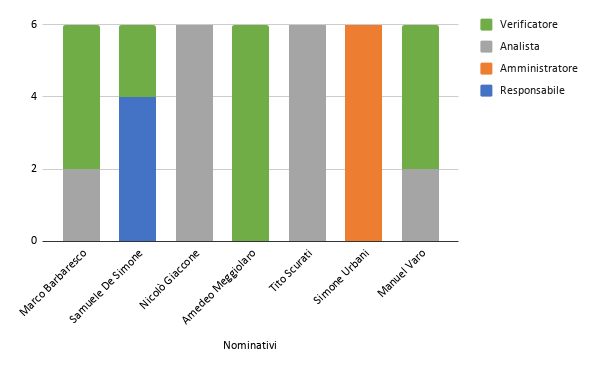
\includegraphics[scale=0.6]{../../../Images/Diagrammi/Istogrammi/ore requisiti.png}
    \centering
    \caption{Istogramma della ripartizione di ore per ruolo in Consolidamento dei requisiti}
\end{figure}

\subsubsection{Prospetto economico}
In questa fase i costi da affrontare per ogni ruolo sono i seguenti:
\begin{center}
    \begin{table}[ht!]
        \centering
        \caption{Prospetto dei costi per ruolo della fase di Consolidamento dei requisiti}
        \vspace{5px}
        \rowcolors{2}{logo!10}{logo!40}
        \renewcommand{\arraystretch}{1.8}
        \begin{tabular}{p{75px} p{20px} p{50px}}
            \rowcolor{logo!70} \textbf{Ruolo} & \textbf{Ore} & \textbf{Costo} \\
            Responsabile                      & 4            & 120,00\EURdig  \\
            Amministratore                    & 6            & 120,00\EURdig  \\
            Analista                          & 16           & 400,00\EURdig  \\
            Progettista                       & -            & -              \\
            Programmatore                     & -            & -              \\
            Verificatore                      & 16           & 240,00\EURdig  \\
            Totale                            & 42           & 880,00\EURdig  \\
        \end{tabular}
    \end{table}
\end{center}
\pagebreak

I dati appena descritti si possono riassumere nel seguente areogramma:
\begin{figure}[!h]
    \vspace{5px}
    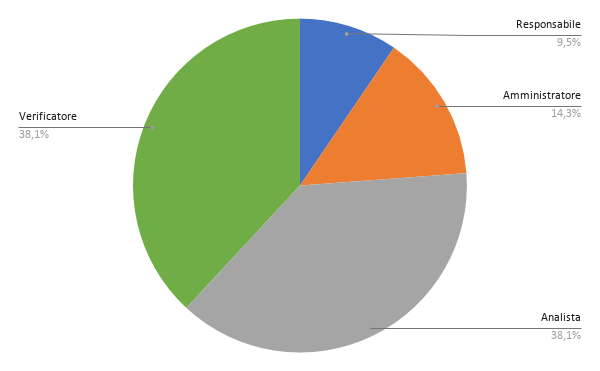
\includegraphics[scale=0.5]{../../../Images/Diagrammi/Diagramma a torta/ore requisiti.png}
    \centering
    \caption{Areogramma della ripartizione di ore per ruolo in Consolidamento dei requisiti}
\end{figure}



\subsection{Fase di Progettazione architetturale}
\subsubsection{Prospetto orario}
Durante il periodo di Progettazione architetturale la ripartizione oraria dei ruoli sarà la seguente:
\begin{center}
    \begin{table}[ht!]
        \centering
        \caption{Distribuzione delle ore della fase di Progettazione architetturale}
        \vspace{5px}
        \rowcolors{2}{logo!10}{logo!40}
        \renewcommand{\arraystretch}{1.8}
        \begin{tabular}{p{100px} p{20px} p{20px} p{20px} p{20px} p{20px} p{20px} p{50px} }
            \rowcolor{logo!70} \textbf{Nominativo} & \textbf{Re} & \textbf{Am} & \textbf{An} & \textbf{Pt} & \textbf{Pr} & \textbf{Ve} & \textbf{Ore totali} \\
            Marco Barbaresco                       & -           & -           & 6           & 13          & 5           & 4           & 28                  \\
            Samuele De Simone                      & -           & -           & 10          & -           & 6           & 12          & 28                  \\
            Nicolò Giaccone                        & -           & 7           & -           & 15          & 6           & -           & 28                  \\
            Amedeo Meggiolaro                      & 5           & -           & -           & 12          & 3           & 8           & 28                  \\
            Tito Scutari                           & 10          & 7           & -           & 11          & -           & -           & 28                  \\
            Simone Urbani                          & -           & -           & 6           & 12          & -           & 10          & 28                  \\
            Manuel Varo                            & -           & 5           & 8           & -           & 6           & 9           & 28                  \\
            Ore totali di ruolo                    & 15          & 19          & 30          & 63          & 26          & 43          & 196                 \\
        \end{tabular}
    \end{table}
\end{center}
\pagebreak

I dati appena descritti si possono riassumere nel seguente istogramma:
\begin{figure}[!h]
    \vspace{5px}
    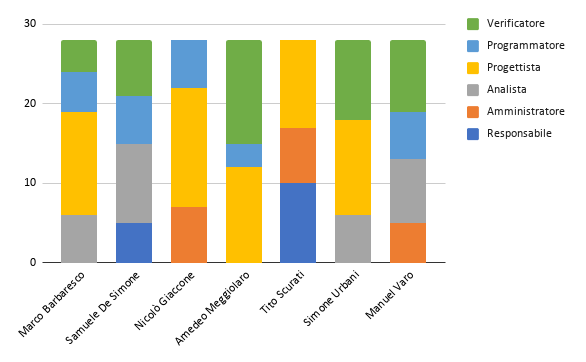
\includegraphics[scale=0.6]{../../../Images/Diagrammi/Istogrammi/ore architettura.png}
    \centering
    \caption{Istogramma della suddivisione di ore per ruolo in Progettazione architetturale}
\end{figure}

\subsubsection{Prospetto economico}
In questa fase i costi da affrontare per ogni ruolo sono i seguenti:
\begin{center}
    \begin{table}[ht!]
        \centering
        \caption{Prospetto dei costi per ruolo della fase di Progettazione architetturale}
        \vspace{5px}
        \rowcolors{2}{logo!10}{logo!40}
        \renewcommand{\arraystretch}{1.8}
        \begin{tabular}{p{75px} p{20px} p{50px}}
            \rowcolor{logo!70} \textbf{Ruolo} & \textbf{Ore} & \textbf{Costo}  \\
            Responsabile                      & 15           & 450,00\EURdig   \\
            Amministratore                    & 19           & 380,00\EURdig   \\
            Analista                          & 30           & 750,00\EURdig   \\
            Progettista                       & 63           & 1.368,00\EURdig \\
            Programmatore                     & 26           & 390,00\EURdig   \\
            Verificatore                      & 43           & 645,00\EURdig   \\
            Totale                            & 196          & 4.001,00\EURdig \\
        \end{tabular}
    \end{table}
\end{center}
\pagebreak

I dati appena descritti si possono riassumere nel seguente areogramma:
\begin{figure}[!h]
    \vspace{5px}
    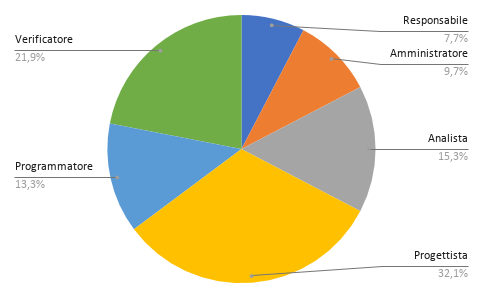
\includegraphics[scale=0.5]{../../../Images/Diagrammi/Diagramma a torta/ore architettura.png}
    \centering
    \caption{Areogramma della suddivisione di ore per ruolo in Progettazione architetturale}
\end{figure}


\subsection{Fase di Progettazione di dettaglio e codifica}
\subsubsection{Prospetto orario}
Per il periodo di Progettazione di dettaglio e codifica la ripartizione oraria dei ruoli sarà la seguente:
\begin{center}
    \begin{table}[ht!]
        \centering
        \caption{Distribuzione delle ore della fase di Progettazione di dettaglio e codifica}
        \vspace{5px}
        \rowcolors{2}{logo!10}{logo!40}
        \renewcommand{\arraystretch}{1.8}
        \begin{tabular}{p{100px} p{20px} p{20px} p{20px} p{20px} p{20px} p{20px} p{50px} }
            \rowcolor{logo!70} \textbf{Nominativo} & \textbf{Re} & \textbf{Am} & \textbf{An} & \textbf{Pt} & \textbf{Pr} & \textbf{Ve} & \textbf{Ore totali} \\
            Marco Barbaresco                       & 9           & -           & -           & 14          & 12          & 15          & 50                  \\
            Samuele De Simone                      & -           & 8           & -           & 18          & 13          & 11          & 50                  \\
            Nicolò Giaccone                        & 8           & -           & -           & 8           & 20          & 14          & 50                  \\
            Amedeo Meggiolaro                      & 6           & 5           & -           & 9           & 12          & 18          & 50                  \\
            Tito Scutari                           & -           & 9           & -           & 14          & 18          & 9           & 50                  \\
            Simone Urbani                          & 8           & -           & -           & 14          & 16          & 12          & 50                  \\
            Manuel Varo                            & -           & 12          & -           & 13          & 9           & 16          & 50                  \\
            Ore totali di ruolo                    & 31          & 34          & 0           & 90          & 100         & 95          & 350                 \\
        \end{tabular}
    \end{table}
\end{center}
\pagebreak

I dati appena descritti si possono riassumere nel seguente istogramma:
\begin{figure}[!h]
    \vspace{5px}
    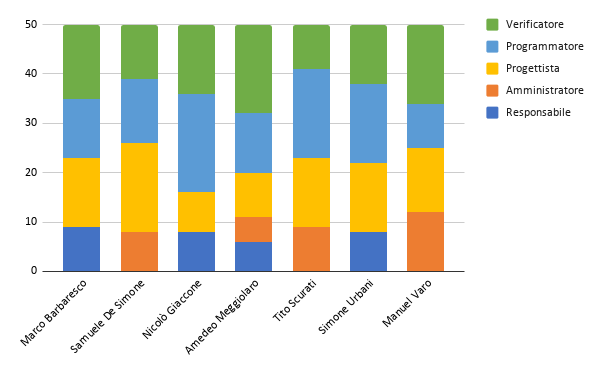
\includegraphics[scale=0.6]{../../../Images/Diagrammi/Istogrammi/ore codifica.png}
    \centering
    \caption{Istogramma della suddivisione di ore per ruolo in Progettazione di dettaglio e codifica}
\end{figure}
\subsubsection{Prospetto economico}
In questa fase i costi da affrontare per ogni ruolo sono i seguenti:
\begin{center}
    \begin{table}[ht!]
        \centering
        \caption{Prospetto dei costi per ruolo della fase di Progettazione di dettaglio e codifica}
        \vspace{5px}
        \rowcolors{2}{logo!10}{logo!40}
        \renewcommand{\arraystretch}{1.8}
        \begin{tabular}{p{75px} p{20px} p{50px}}
            \rowcolor{logo!70} \textbf{Ruolo} & \textbf{Ore} & \textbf{Costo}  \\
            Responsabile                      & 31           & 930,00\EURdig   \\
            Amministratore                    & 34           & 680,00\EURdig   \\
            Analista                          & -            & -               \\
            Progettista                       & 90           & 1.980,00\EURdig \\
            Programmatore                     & 100          & 1.500,00\EURdig \\
            Verificatore                      & 95           & 1.425,00\EURdig \\
            Totale                            & 350          & 6.515,00\EURdig \\
        \end{tabular}
    \end{table}
\end{center}
\pagebreak

I dati appena descritti si possono riassumere nel seguente areogramma:
\begin{figure}[!h]
    \vspace{5px}
    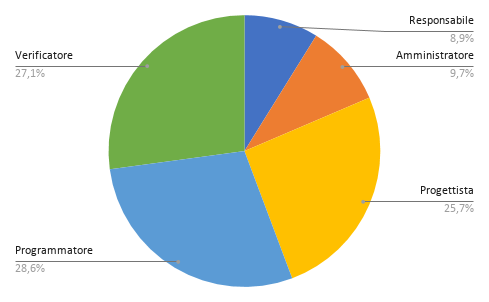
\includegraphics[scale=0.5]{../../../Images/Diagrammi/Diagramma a torta/ore codifica.png}
    \centering
    \caption{Areogramma della suddivisione di ore per ruolo in Progettazione di dettaglio e codifica}
\end{figure}



\subsection{Fase di Validazione e collaudo}
\subsubsection{Prospetto orario}
Per il periodo di Validazione e collaudo la ripartizione oraria dei ruoli sarà la seguente:
\begin{center}
    \begin{table}[ht!]
        \centering
        \caption{Distribuzione delle ore della fase di Validazione e collaudo}
        \vspace{5px}
        \rowcolors{2}{logo!10}{logo!40}
        \renewcommand{\arraystretch}{1.8}
        \begin{tabular}{p{100px} p{20px} p{20px} p{20px} p{20px} p{20px} p{20px} p{50px} }
            \rowcolor{logo!70} \textbf{Nominativo} & \textbf{Re} & \textbf{Am} & \textbf{An} & \textbf{Pt} & \textbf{Pr} & \textbf{Ve} & \textbf{Ore totali} \\
            Marco Barbaresco                       & -           & 8           & -           & 2           & -           & 10          & 20                  \\
            Samuele De Simone                      & 4           & -           & -           & -           & 7           & 9           & 20                  \\
            Nicolò Giaccone                        & -           & 5           & -           & 6           & -           & 9           & 20                  \\
            Amedeo Meggiolaro                      & -           & -           & -           & 12          & 8           & -           & 20                  \\
            Tito Scutari                           & 6           & -           & -           & -           & 12          & 2           & 20                  \\
            Simone Urbani                          & -           & 6           & -           & -           & 10          & 4           & 20                  \\
            Manuel Varo                            & 10          & -           & -           & -           & 4           & 6           & 20                  \\
            Ore totali di ruolo                    & 20          & 19          & 0           & 20          & 41          & 40          & 140                 \\
        \end{tabular}
    \end{table}
\end{center}
\pagebreak

I dati appena descritti si possono riassumere nel seguente istogramma:
\begin{figure}[!h]
    \vspace{5px}
    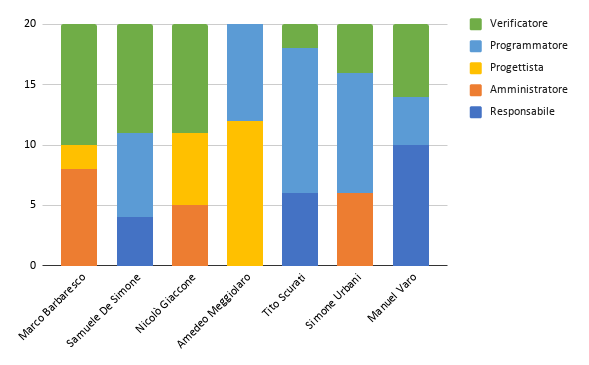
\includegraphics[scale=0.6]{../../../Images/Diagrammi/Istogrammi/ore validificazione.png}
    \centering
    \caption{Istogramma della suddivisione di ore per ruolo in Validazione e collaudo}
\end{figure}
\subsubsection{Prospetto economico}
In questa fase i costi da affrontare per ogni ruolo sono i seguenti:

\begin{center}
    \begin{table}[ht!]
        \centering
        \caption{Prospetto dei costi per ruolo della fase di Validazione e collaudo}
        \vspace{5px}
        \rowcolors{2}{logo!10}{logo!40}
        \renewcommand{\arraystretch}{1.8}
        \begin{tabular}{p{75px} p{20px} p{50px}}
            \rowcolor{logo!70} \textbf{Ruolo} & \textbf{Ore} & \textbf{Costo}  \\
            Responsabile                      & 20           & 600,00\EURdig   \\
            Amministratore                    & 19           & 380,00\EURdig   \\
            Analista                          & -            & -               \\
            Progettista                       & 20           & 440,00\EURdig   \\
            Programmatore                     & 41           & 615,00\EURdig   \\
            Verificatore                      & 40           & 600,00\EURdig   \\
            Totale                            & 140          & 2.635,00\EURdig \\
        \end{tabular}
    \end{table}
\end{center}
\pagebreak

I dati appena descritti si possono riassumere nel seguente areogramma:
\begin{figure}[!h]
    \vspace{5px}
    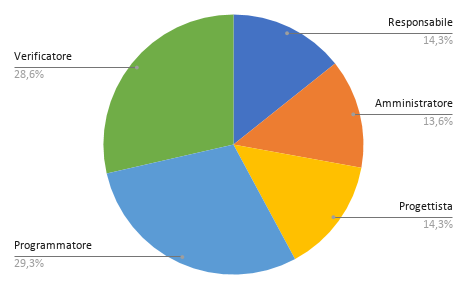
\includegraphics[scale=0.5]{../../../Images/Diagrammi/Diagramma a torta/ore validificazione.png}
    \centering
    \caption{Areogramma della suddivisione di ore per ruolo in Validazione e collaudo}
\end{figure}


\subsection{Riepilogo}
\subsubsection{Ore totali}
\subsubsubsection{Suddivisione lavoro}
Nella tabella sottostante è riportato il totale delle ore del progetto, sono presenti sia le ore d'investimento che quelle rendicontate a carico del committente:
\begin{center}
    \begin{table}[ht!]
        \centering\caption{Distribuzione delle ore totali d'investimento e rendicontate}
        \vspace{5px}
        \rowcolors{2}{logo!10}{logo!40}
        \renewcommand{\arraystretch}{1.8}
        \begin{tabular}{p{100px} p{20px} p{20px} p{20px} p{20px} p{20px} p{20px} p{50px} }
            \rowcolor{logo!70} \textbf{Nominativo} & \textbf{Re} & \textbf{Am} & \textbf{An} & \textbf{Pt} & \textbf{Pr} & \textbf{Ve} & \textbf{Ore totali} \\
            Marco Barbaresco                       & 9           & 18          & 18          & 29          & 17          & 48          & 139                 \\
            Samuele De Simone                      & 16          & 8           & 27          & 18          & 26          & 44          & 139                 \\
            Nicolò Giaccone                        & 8           & 19          & 27          & 29          & 26          & 30          & 139                 \\
            Amedeo Meggiolaro                      & 11          & 5           & 18          & 33          & 23          & 49          & 139                 \\
            Tito Scutari                           & 16          & 24          & 18          & 25          & 30          & 26          & 139                 \\
            Simone Urbani                          & 14          & 22          & 14          & 26          & 26          & 37          & 139                 \\
            Manuel Varo                            & 17          & 17          & 22          & 13          & 19          & 51          & 139                 \\
            Ore totali di ruolo                    & 91          & 113         & 144         & 173         & 167         & 285         & 973                 \\
        \end{tabular}
    \end{table}
\end{center}
\pagebreak
Una rappresentazione visiva della suddivisione oraria viene data dal seguente grafico:

\begin{figure}[!h]
    \vspace{5px}
    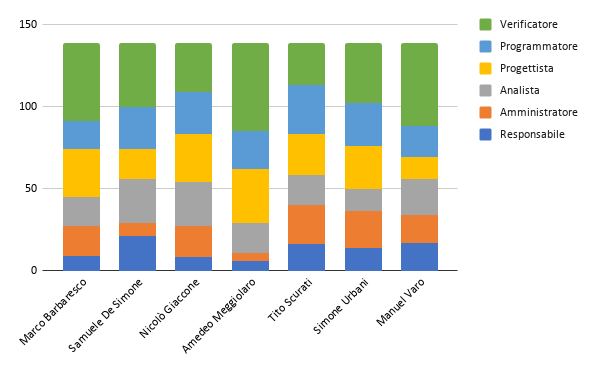
\includegraphics[scale=0.6]{../../../Images/Diagrammi/Istogrammi/ore totali.png}
    \centering
    \caption{Istogramma della suddivisione delle ore totali d'investimento e rendicontate}
\end{figure}

\subsubsubsection{Prospetto economico}
I costi da affrontare per ogni ruolo sono i seguenti:
\begin{center}
    \begin{table}[ht!]
        \centering
        \caption{Prospetto dei costi totale delle ore d'investimento e rendicontate}
        \vspace{5px}
        \rowcolors{2}{logo!10}{logo!40}
        \renewcommand{\arraystretch}{1.8}
        \begin{tabular}{p{75px} p{20px} p{50px}}
            \rowcolor{logo!70} \textbf{Ruolo} & \textbf{Ore} & \textbf{Costo}   \\
            Responsabile                      & 91           & 2.730,00\EURdig  \\
            Amministratore                    & 113          & 2.260,00\EURdig  \\
            Analista                          & 144          & 3.600,00\EURdig  \\
            Progettista                       & 173          & 3.806,00\EURdig  \\
            Programmatore                     & 167          & 2.505,00\EURdig  \\
            Verificatore                      & 285          & 4.275,00\EURdig  \\
            Totale                            & 973          & 19.176,00\EURdig \\
        \end{tabular}
    \end{table}
\end{center}
\pagebreak
dati ottenuti si possono riassumere nel seguente areogramma:
\begin{figure}[!h]
    \vspace{5px}
    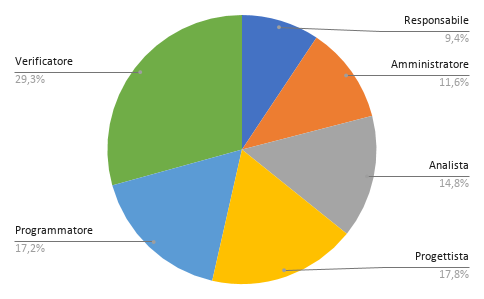
\includegraphics[scale=0.5]{../../../Images/Diagrammi/Diagramma a torta/ore totali.png}
    \centering
    \caption{Areogramma dei costi delle ore totali d'investimento e rendicontate}
\end{figure}

\subsubsection{Ore rendicontate}
\subsubsubsection{Suddivisione lavoro}
Le ore rendicontate sono riportate nella seguente tabella:
\begin{center}
    \begin{table}[ht!]
        \centering
        \caption{Distribuzione delle ore rendicontate}
        \vspace{5px}
        \rowcolors{2}{logo!10}{logo!40}
        \renewcommand{\arraystretch}{1.8}
        \begin{tabular}{p{100px} p{20px} p{20px} p{20px} p{20px} p{20px} p{20px} p{50px} }
            \rowcolor{logo!70} \textbf{Nominativo} & \textbf{Re} & \textbf{Am} & \textbf{An} & \textbf{Pt} & \textbf{Pr} & \textbf{Ve} & \textbf{Ore totali} \\
            Marco Barbaresco                       & 9           & 8           & 8           & 29          & 17          & 33          & 104                 \\
            Samuele De Simone                      & 8           & 8           & 10          & 18          & 26          & 34          & 104                 \\
            Nicolò Giaccone                        & 8           & 12          & 6           & 29          & 26          & 23          & 104                 \\
            Amedeo Meggiolaro                      & 11          & 5           & 0           & 33          & 23          & 32          & 104                 \\
            Tito Scutari                           & 16          & 16          & 6           & 25          & 30          & 11          & 104                 \\
            Simone Urbani                          & 8           & 12          & 6           & 26          & 26          & 26          & 104                 \\
            Manuel Varo                            & 10          & 17          & 10          & 13          & 19          & 35          & 104                 \\
            Ore totali di ruolo                    & 70          & 78          & 46          & 173         & 167         & 194         & 728                 \\
        \end{tabular}
    \end{table}
\end{center}
\pagebreak
Una rappresentazione visiva della suddivisione oraria viene data dal seguente grafico:
\begin{figure}[!h]
    \vspace{5px}
    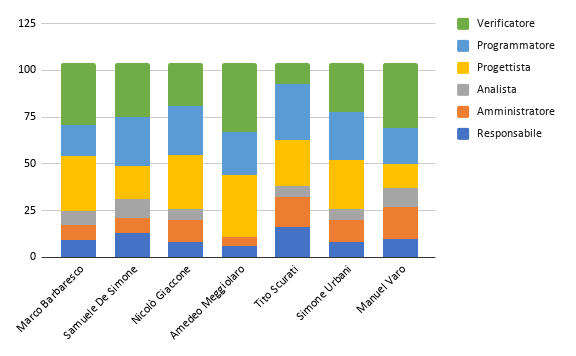
\includegraphics[scale=0.6]{../../../Images/Diagrammi/Istogrammi/ore rendicontate.png}
    \centering
    \caption{Istogramma della suddivisione delle ore rendicontate}
\end{figure}

\subsubsubsection{Prospetto economico}
Il totale rendicontato dei costi da affrontare per ogni ruolo è:

\begin{center}
    \begin{table}[ht!]
        \centering
        \caption{Prospetto dei costi delle ore rendicontate}
        \vspace{5px}
        \rowcolors{2}{logo!10}{logo!40}
        \renewcommand{\arraystretch}{1.8}
        \begin{tabular}{p{75px} p{20px} p{50px}}
            \rowcolor{logo!70} \textbf{Ruolo} & \textbf{Ore} & \textbf{Costo}   \\
            Responsabile                      & 70           & 2.100,00\EURdig  \\
            Amministratore                    & 78           & 1.560,00\EURdig  \\
            Analista                          & 46           & 1.150,00\EURdig  \\
            Progettista                       & 173          & 3.806,00\EURdig  \\
            Programmatore                     & 167          & 2.505,00\EURdig  \\
            Verificatore                      & 194          & 2.910,00\EURdig  \\
            Totale                            & 728          & 14.031,00\EURdig \\
        \end{tabular}
    \end{table}
\end{center}
\pagebreak
dati ottenuti si possono riassumere nel seguente areogramma:
\begin{figure}[!h]
    \vspace{5px}
    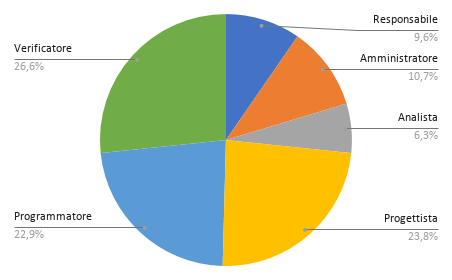
\includegraphics[scale=0.5]{../../../Images/Diagrammi/Diagramma a torta/ore rendicontate.png}
    \centering
    \caption{Areogramma delle ore rendicontate per ruolo}
\end{figure}

\subsection{Conclusioni}
Considerando solamente le ore rendicontate, il costo del progetto è di: 14.031,00\EURdig.